\documentclass[a4paper,12pt]{article}

\usepackage[russian]{babel} % Язык документа

% Подключаем fontspec для управления шрифтами
\usepackage{fontspec}

% Выбираем шрифты с поддержкой кириллицы (установленные в системе)
\setmainfont{CMU Serif} % или "Times New Roman", или "Linux Libertine O"
\setsansfont{CMU Sans Serif}
\setmonofont{CMU Typewriter Text}

\usepackage{geometry}
\geometry{left=30mm, right=10mm, top=20mm, bottom=20mm}

\usepackage{setspace}
\onehalfspacing
\setlength{\parindent}{15mm}

\usepackage{graphicx}
\usepackage{caption}
\usepackage{booktabs}
\usepackage{amsmath}
\usepackage{tocloft}
\usepackage{titlesec}
\usepackage{float}
\usepackage{hyperref}
\usepackage{listings}
\usepackage{xcolor}

\lstset{
	language=Python,
	basicstyle=\ttfamily\small,
	keywordstyle=\color{blue}\bfseries,
	stringstyle=\color{red},
	commentstyle=\color{green!50!black},
	numbers=left,
	numberstyle=\tiny,
	stepnumber=1,
	numbersep=5pt,
	showspaces=false,
	showstringspaces=false,
	frame=none,
	breaklines=true,
	breakatwhitespace=true,
	tabsize=2,
	columns=fullflexible,
	mathescape=false,
}

\titleformat{\section}{\normalfont\bfseries}{\thesection}{1em}{}
\titleformat{\subsection}{\normalfont\bfseries}{\thesubsection}{1em}{}

% Форматирование титульной страницы
\begin{document}

\begin{titlepage}
	\vspace*{1cm}
	{\small
		\begin{center}
			МИНИСТЕРСТВО НАУКИ И ВЫСШЕГО ОБРАЗОВАНИЯ РОССИЙСКОЙ ФЕДЕРАЦИИ\\
			ФЕДЕРАЛЬНОЕ ГОСУДАРСТВЕННОЕ АВТОНОМНОЕ ОБРАЗОВАТЕЛЬНОЕ УЧРЕЖДЕНИЕ ВЫСШЕГО ОБРАЗОВАНИЯ\\
			\textbf{НАЦИОНАЛЬНЫЙ ИССЛЕДОВАТЕЛЬСКИЙ ТОМСКИЙ ПОЛИТЕХНИЧЕСКИЙ УНИВЕРСИТЕТ}
		\end{center}
	}
	\vspace{0.5cm}
	\begin{center}
		Инженерная школа информационных технологий и робототехники\\
		Отделение информационных технологий\\
		Направление: 09.04.01 Искусственный интеллект и машинное обучение
	\end{center}
	\vspace{1cm}
	\begin{center}
		\textbf{ОТЧЁТ ПО ПРАКТИЧЕСКОЙ РАБОТЕ}
	\end{center}
	\begin{center}
		по дисциплине: Нейроэволюционные вычисления
	\end{center}
	\vspace{0.5cm}
	% Добавление "Вариант 21" по центру
	\begin{center}
		\textbf{Вариант 1}
	\end{center}
	\begin{center}
		на тему: Реализация алгоритма нейроэволюции NEAT для непрерывного контроля в среды Bipedal Walker
	\end{center}
	\vspace{1cm}
	
	% Двухколоночное расположение
	\begin{tabular}{p{0.3\textwidth} p{0.35\textwidth} p{0.3\textwidth}}
		\textbf{Выполнил:} & студент гр. 8ВМ42 \newline Агарков Д.А.& 09.06.2025\\
		& & \\
		\textbf{Проверил:} & к.т.н., Доцент ОИТ ИШИТР \newline Григорьев Д.С. & 09.06.2025\end{tabular}
	\vfill
	\begin{center}
		Томск – 2025
	\end{center}
\end{titlepage}


% Оглавление
\tableofcontents
\setcounter{page}{2}
\newpage

% Настройка форматирования разделов и интервалов
\titleformat{\section}{\normalfont\bfseries}{\thesection}{1em}{}
\titleformat{\subsection}{\normalfont\bfseries}{\thesubsection}{1em}{}
\setlength{\parindent}{15mm}
\onehalfspacing

% Раздел 1: Введение
\section{Введение}
Нейроэволюция — это подход к обучению нейронных сетей, основанный на принципах эволюционного отбора. В отличие от традиционных методов, таких как градиентное обучение или обратное распространение ошибки, нейроэволюционные алгоритмы не требуют наличия производных целевой функции и способны эффективно работать в условиях негладких, стохастических и дискретных сред. Это делает нейроэволюцию особенно перспективной в задачах, где градиентные методы не применимы или дают нестабильные результаты.

Одним из наиболее известных и мощных алгоритмов нейроэволюции является \textbf{NEAT} (NeuroEvolution of Augmenting Topologies), предложенный Кеном Стэнли. Его ключевая особенность — это одновременная эволюция как весов, так и структуры нейронной сети. Алгоритм начинает обучение с минимально возможной топологии (обычно — только входной и выходной слои) и постепенно усложняет сеть по мере необходимости, добавляя скрытые нейроны и новые связи. Такой подход позволяет избежать переобучения на ранних стадиях и эффективно исследовать пространство решений.

NEAT реализует ряд уникальных механизмов:
\begin{itemize}
  \item \textbf{Исторические метки (innovation numbers)} — позволяют отслеживать происхождение связей и синхронизировать гены при скрещивании сетей с разной архитектурой;
  \item \textbf{Мутации структуры} — добавление новых нейронов и связей во время эволюции;
  \item \textbf{Специализация (speciation)} — деление популяции на виды, конкуренция происходит внутри вида, а не между всеми особями сразу, что защищает потенциально полезные новшества от преждевременного отбора.
\end{itemize}

В данной работе рассматривается применение алгоритма NEAT к задаче непрерывного управления в симулированной среде \texttt{BipedalWalker-v3} из библиотеки Gymnasium. Это среда с непрерывным пространством действий, в которой агент должен научиться координировать движение ног для устойчивой ходьбы по неровной поверхности. Данная задача требует от алгоритма способности строить эффективные стратегии управления, которые опираются как на сенсорные данные, так и на внутреннюю динамику сети.

\textbf{Цель работы} — реализовать алгоритм NEAT и обучить нейронную сеть с развивающейся архитектурой для эффективного управления агентом в среде \texttt{BipedalWalker-v3}, выполнив:
\begin{itemize}
  \item реализацию и описание механизмов NEAT (кодирования, мутации, скрещивания, специализации);
  \item визуализацию структуры сети на разных этапах обучения;
  \item анализ сходимости по метрикам среды (например, reward);
  \item сохранение и загрузку состояния сети для воспроизводимости.
\end{itemize}


\newpage
% Раздел 2: Описание алгоритма
\section{Описание используемого алгоритма}

\subsection{Принципы работы NEAT (NeuroEvolution of Augmenting Topologies)}
Алгоритм NEAT (NeuroEvolution of Augmenting Topologies), предложенный Кеном Стэнли, представляет собой метод нейроэволюционного обучения, в котором происходит одновременная эволюция как весов, так и архитектуры нейронной сети. В отличие от традиционных генетических алгоритмов с фиксированной структурой генома, NEAT динамически наращивает сложность сети, начиная с простой топологии и постепенно добавляя новые нейроны и связи по мере необходимости.

\paragraph{Основные механизмы алгоритма NEAT:}
\begin{itemize}
    \item \textbf{Геномное представление:} нейронная сеть кодируется списком генов-связей с указанием входного/выходного нейрона, веса, статуса активности и номера инновации;
    \item \textbf{Исторические метки (innovation numbers):} каждая новая структура связи получает уникальный идентификатор, что позволяет корректно проводить скрещивание между сетями с различной топологией;
    \item \textbf{Эволюционное наращивание:} в процессе мутации возможны не только изменения весов, но и добавление новых нейронов или связей;
    \item \textbf{Специализация (speciation):} популяция особей разбивается на виды, внутри которых происходит локальная конкуренция, что предотвращает преждевременное вымирание редких, но перспективных мутаций;
    \item \textbf{Скрещивание с выравниванием генов:} потомки формируются из совпадающих по инновациям генов, а также из несовпадающих генов наиболее приспособленного родителя.
\end{itemize}

\subsection{Структура сети}
В данной реализации алгоритма NEAT используется нейронная сеть с архитектурой \texttt{feedforward}, где информация передается от входных нейронов через скрытые нейроны к выходным, без рекуррентных связей. Эта структура подходит для задач, где необходимо моделировать зависимости между входами и выходами в динамическом и непрерывном контексте, как в случае с \texttt{BipedalWalker-v3}.

Нейронная сеть состоит из нескольких ключевых компонентов:
\begin{itemize}
\item \textbf{Входной слой:} состоит из нейронов, количество которых соответствует размерности входных данных. Для задачи \texttt{BipedalWalker-v3} это 24 признака, описывающих состояние агента и окружающей среды.
    \item \textbf{Скрытые слои:} количество скрытых нейронов не ограничено и может изменяться в ходе эволюции. В начале сети скрытые нейроны отсутствуют, и они добавляются только по мере необходимости в процессе мутации.
    \item \textbf{Выходной слой:} состоит из нейронов, количество которых соответствует количеству управляющих сигналов. В задаче управления \texttt{BipedalWalker-v3} это 4 выхода, которые контролируют действия агента (например, управление движением ног).
\end{itemize}

\paragraph{Особенности структуры:}
\begin{itemize}
\item \textbf{Отсутствие рекуррентных связей:} структура сети предполагает только прямое распространение информации от входных нейронов к выходным. Это обеспечивает простоту архитектуры и быстрое обучение на начальных этапах.
    \item \textbf{Динамическое расширение сети:} количество нейронов и связей в сети может изменяться во время эволюции. Изначально сеть имеет минимальную структуру, состоящую только из входных и выходных нейронов, но по мере эволюции могут добавляться новые скрытые нейроны и связи между ними.
    \item \textbf{Мутации структуры:} при мутации сети могут быть добавлены новые нейроны и связи. Эти мутации происходят случайным образом с определённой вероятностью, что позволяет гибко изменять архитектуру сети в ответ на изменяющиеся требования задачи.
\end{itemize}

\subsection{Логика разбиения на подпопуляции, эволюция на уровне нейрона}
В алгоритме NEAT ключевым моментом является разделение популяции на подпопуляции, каждая из которых отвечает за эволюцию нейронов скрытого слоя. Это разделение способствует специализации нейронов и позволяет каждому нейрону оптимизировать свои параметры (веса входных и выходных связей) независимо от остальных, что повышает эффективность алгоритма.
\begin{itemize}
\item \textbf{Подпопуляция для каждого нейрона:} Каждому нейрону скрытого слоя соответствует своя подпопуляция. Каждая особь в подпопуляции — это набор параметров для нейрона, включающий веса входных связей, веса выходных связей, а также, если требуется, смещения. Таким образом, каждый нейрон представляется как самостоятельная эволюционная единица, которая может изменяться и развиваться независимо от других нейронов.
	
	\item \textbf{Формирование команд для оценки:} Для оценки приспособленности нейронов создаются \textit{команды}, которые представляют собой нейронные сети, сформированные из случайных представителей всех подпопуляций. Это означает, что каждый агент оценивается не по отдельности, а как часть группы, где его нейрон взаимодействует с нейронами из других подпопуляций. Это помогает улучшить качество обучения и способствует более разнообразным и сильным решениям.
	
	\item \textbf{Оценка приспособленности нейронов:} Оценка нейрона в подпопуляции происходит на основе кумулятивного фитнеса, то есть его приспособленность определяется как сумма результатов всех команд, в которых этот нейрон принимал участие. Каждая особь должна быть использована в сети минимум определённое количество раз, например, 10 раз. Это обеспечивает более надёжную оценку его способности вносить вклад в решение задачи.
	
	\item \textbf{Специализация нейронов:} Благодаря эволюции на уровне нейрона, каждый нейрон постепенно становится специализированным, решая определённые подзадачи, такие как обработка специфических частей информации или управление отдельными аспектами задачи. Это приводит к улучшению общей производительности сети, так как каждый нейрон адаптируется и оптимизируется под свою функцию. Разделение популяции на подпопуляции также предотвращает переобучение, обеспечивая разнообразие в возможных решениях и архитектурах сети.
\end{itemize}

\subsection{Этапы алгоритма NEAT}
Алгоритм NEAT состоит из нескольких ключевых этапов, которые помогают эффективно эволюционировать нейронные сети. В каждом поколении популяция агентов проходит через этапы оценки, мутации, скрещивания и специализации, что способствует улучшению качества решения задачи и созданию устойчивых стратегий управления:
\begin{enumerate}
    \item \textbf{Инициализация популяции:}
    \begin{itemize}
        \item Создаётся начальная популяция агентов с минимальными структурами нейронных сетей. На этом этапе каждый агент состоит только из входных и выходных нейронов, и сети ещё не имеют скрытых слоёв или дополнительных связей.
        \item Каждому агенту присваиваются случайные веса связей между нейронами, и они начинают эволюционировать с равными шансами на успех.
    \end{itemize}

    \item \textbf{Оценка приспособленности (fitness evaluation):}
    \begin{itemize}
        \item Каждый агент оценивается в среде. Для этого выполняется несколько эпизодов (например, 10), в которых агент взаимодействует с окружением, выполняет действия, и на основе этих действий получает вознаграждения.
        \item Приспособленность агента определяется суммой полученных вознаграждений в ходе всех эпизодов. Это позволяет оценить, насколько хорошо агент решает поставленную задачу.
    \end{itemize}

    \item \textbf{Специализация (speciation):}
    \begin{itemize}
        \item После того как все агенты были оценены, популяция разделяется на виды в зависимости от схожести их геномов (структуры нейронных сетей). Это делается с помощью расчёта расстояния между генами агентов, которое измеряет различия в топологии и весах их сетей.
        \item Виды помогают сохранять разнообразие в популяции и предотвращают быструю конкуренцию между агентами с радикально разными структурами сетей, обеспечивая условия для развития новых, более эффективных сетей.
    \end{itemize}

    \item \textbf{Скрещивание (crossover):}
    \begin{itemize}
        \item Для каждого вида выбираются родители, которые будут участвовать в скрещивании. При этом выбираются агенты с наибольшими значениями приспособленности.
        \item На основе генов выбранных родителей создаются потомки. При скрещивании гены с одинаковыми номерами инноваций могут быть объединены случайным образом, в зависимости от вероятности.
        \item Новые агенты создаются путём комбинирования весов и структурных изменений от родителей, что позволяет генерировать новые вариации, способные решать задачу лучше.
    \end{itemize}

    \item \textbf{Мутация (mutation):}
    \begin{itemize}
        \item Мутация является ключевым этапом, позволяющим добавлять новые нейроны и связи в сети. Она происходит случайным образом и может затрагивать как веса существующих связей, так и структуру сети.
        \item Возможные мутации включают: добавление новых нейронов (что увеличивает сложность сети), добавление новых связей между нейронами, изменение веса существующих связей.
        \item Вероятность и тип мутации зависят от конфигурации алгоритма (например, вероятность изменения весов или добавления новых связей).
    \end{itemize}

    \item \textbf{Отбор (selection):}
    \begin{itemize}
        \item После скрещивания и мутации популяция обновляется, и остаются только лучшие особи (с наибольшим фитнесом). Это позволяет сохранять в популяции наиболее успешных агентов.
        \item Отбор может быть как жестким (отбираются только лучшие агенты), так и более мягким, с возможностью оставить определённое количество менее приспособленных агентов для дальнейшего улучшения.
    \end{itemize}

    \item \textbf{Повторение:}
    \begin{itemize}
        \item Шаги 2-5 повторяются несколько раз (в течение заданного числа поколений или до достижения заданного уровня производительности).
        \item По мере повторения этих шагов, сеть будет усложняться и оптимизироваться, улучшая свои способности к решению задачи.
    \end{itemize}

    \item \textbf{Сохранение состояния (optional):}
    \begin{itemize}
        \item Состояние каждого агента и его сети может быть сохранено в файл (например, с помощью сериализации в формат pickle). Это позволяет продолжить обучение с того места, где оно было остановлено, или проанализировать прогресс обучения.
    \end{itemize}
\end{enumerate}

Таким образом, алгоритм NEAT эволюционирует нейронные сети, начиная с простых структур и постепенно добавляя новые нейроны и связи. Благодаря этому методу, агент может адаптировать свою структуру для эффективного решения задачи, постепенно улучшая свою архитектуру и веса на основе опыта в среде.
\newpage
\section{Этапы имплементации}

Реализация алгоритма NEAT для задачи управления в среде \texttt{BipedalWalker-v3} была выполнена на языке Python с использованием библиотеки \texttt{gymnasium} для симуляции среды и \texttt{numpy} для работы с числовыми вычислениями. Алгоритм реализован с нуля, без использования сторонних библиотек или реализаций нейроэволюции, что позволило гибко настроить и адаптировать алгоритм под конкретные требования задачи.

\subsection{Модульная структура кода}

Код организован модульно, что облегчает повторное использование и дальнейшее расширение:
\begin{itemize}
    \item \textbf{NEATConfig:} класс конфигурации, который содержит все основные параметры алгоритма NEAT, такие как размер популяции, вероятность мутаций, параметры мутации весов и структуры сети.
    \item \textbf{Gene:} класс, представляющий отдельную связь в нейронной сети. Каждый ген хранит информацию о связи между двумя нейронами (входном и выходном), весе этой связи и её статусе (включена/выключена).
    \item \textbf{NeuralNetwork:} класс нейронной сети, который управляет созданием сети, её мутацией, а также вычислением выходных данных сети на основе входных данных.
    \item \textbf{Speciation:} класс, реализующий разделение популяции на виды на основе схожести геномов агентов. Он помогает поддерживать разнообразие в популяции и предотвращать слишком быстрый отбор сильнейших агентов.
    \item \textbf{Agent:} класс, представляющий агента в популяции, который взаимодействует с окружающей средой и оценивается на основе полученного вознаграждения.
    \item \textbf{NEAT:} основной класс, реализующий алгоритм NEAT. Он управляет популяцией агентов, координирует процессы мутации, скрещивания и специализации, а также проводит эволюцию популяции.
\end{itemize}

\subsection{Основные этапы реализации}

\paragraph{Инициализация популяции и параметров сети:}

На первом этапе создаётся начальная популяция агентов с минимальными структурами нейронных сетей. Каждый агент состоит из входных и выходных нейронов, инициализированных случайными весами. Веса для связей между нейронами генерируются случайным образом, а структура сети может быть дополнительно изменена в процессе эволюции. На этом этапе сети имеют минимальное количество нейронов, и сложность сети будет увеличиваться по мере добавления новых нейронов и связей в процессе обучения.

\begin{itemize}
	\item[] Реализация в коде:
	\begin{lstlisting}
		self.agents = [Agent(self.env.observation_space.shape[0], self.env.action_space.shape[0]) for _ in range(self.population_size)]
	\end{lstlisting}
\end{itemize}

\paragraph{Оценка приспособленности (fitness evaluation):}

Каждый агент оценивается в среде. Для этого агент взаимодействует с окружением, выполняет действия, и на основе этих действий получает вознаграждения. Приспособленность агента определяется как сумма полученных вознаграждений в ходе всех эпизодов. Агенты выполняют несколько эпизодов в среде, и их фитнес вычисляется на основе их производительности в этих эпизодах.

\begin{itemize}
	\item[] Ключевой фрагмент кода:
	\begin{lstlisting}
		for agent in self.agents:
			agent.fitness = agent.evaluate(self.env)  # Оценка приспособленности
	\end{lstlisting}
\end{itemize}

\paragraph{Специализация популяции (speciation):}

После того как все агенты были оценены, популяция разделяется на виды с помощью класса \texttt{Speciation}. Это разделение помогает сохранить разнообразие популяции и предотвращает преждевременное вытеснение агентов с нестандартной архитектурой. Виды формируются на основе схожести геномов агентов, что способствует эффективной эволюции.

\begin{itemize}
	\item[] Реализация в коде:
	\begin{lstlisting}
		self.speciation.assign_species(self.agents)  # Разбиение популяции на виды
	\end{lstlisting}
\end{itemize}

\paragraph{Скрещивание (crossover):}

После специализации и отбора лучших агентов производится скрещивание. Для каждого вида выбираются два лучших родителя, и на основе их генов создаются потомки. При скрещивании выбираются гены с одинаковыми номерами инноваций, а также случайным образом выбираются гены от родителей с наибольшей приспособленностью.

\begin{itemize}
	\item[] Реализация в коде:
	\begin{lstlisting}
		child = crossover(parent1, parent2)  # Создание потомка через скрещивание
	\end{lstlisting}
\end{itemize}

\paragraph{Мутация (mutation):}

После скрещивания каждый агент подвергается мутации. Мутация может быть как изменением весов существующих связей, так и добавлением новых нейронов и связей. Эти изменения помогают улучшать структуру сети и адаптировать её к новым задачам.

\begin{itemize}
	\item[] Реализация в коде:
	\begin{lstlisting}
		for agent in new_agents:
			agent.network.mutate(self.config)  # Мутация сети
	\end{lstlisting}
\end{itemize}

\paragraph{Отбор (selection):}

После мутации и скрещивания популяция обновляется, и остаются только лучшие агенты с наибольшим фитнесом. Эти агенты составляют новое поколение, которое будет использоваться в следующем цикле эволюции.

\begin{itemize}
	\item[] Реализация в коде:
	\begin{lstlisting}
		self.agents = new_agents  # Обновление популяции
	\end{lstlisting}
\end{itemize}

\paragraph{Повторение (iteration):}

Этапы 2-6 повторяются для каждого поколения. Каждый цикл включает оценку, специализацию, скрещивание, мутацию и отбор, пока не будет достигнут максимальный уровень приспособленности или заданное количество поколений.

\begin{itemize}
	\item[] Реализация в коде:
	\begin{lstlisting}
		for generation in range(max_generations):
			self.evolve()  # Эволюция популяции
	\end{lstlisting}
\end{itemize}

Таким образом, алгоритм NEAT эволюционирует нейронные сети, начиная с простых структур и постепенно добавляя новые нейроны и связи. Это позволяет сети адаптироваться и решать сложные задачи с динамическими изменениями, как в задаче управления агентом в среде \texttt{BipedalWalker-v3}.
\newpage
\section{Целевые метрики}

\subsection{Формальное определение метрики}

Основной целевой метрикой, используемой для оценки эффективности агента в алгоритме NEAT, является \textbf{среднее суммарное вознаграждение за эпизод} (average episodic reward), которое вычисляется как:

\[
R_{\text{avg}} = \frac{1}{N} \sum_{i=1}^{N} R_i
\]

где:
\begin{itemize}
    \item $N$ — количество эпизодов оценки,
    \item $R_i$ — суммарное вознаграждение за $i$-й эпизод.
\end{itemize}

Эта метрика помогает измерить, насколько хорошо агент справляется с задачей в процессе обучения, и позволяет отслеживать прогресс по мере эволюции популяции.

\subsection{Целевая метрика в контексте NEAT}

В контексте NEAT вознаграждение агенту дается за его действия в среде. Агент, который обучается в такой среде, как \texttt{BipedalWalker-v3}, получает вознаграждения, зависящие от нескольких факторов: стабильности, эффективности и скорости выполнения задачи.

Целевая метрика, которая определяется через суммарное вознаграждение, может быть расширена для оценки успешности обучения с учётом таких параметров как:
\begin{itemize}
    \item \textbf{Эффективность использования сети:} метрика учитывает, насколько хорошо нейронная сеть, эволюционирующая по мере популяции, может принимать решения для выполнения задачи.
    \item \textbf{Комплексность структуры сети:} увеличение сложности сети через добавление новых нейронов и связей будет сопровождаться улучшением целевой метрики, если добавление новых элементов помогает решать задачу.
    \item \textbf{Скорость обучения:} как быстро агент достигает хороших значений вознаграждения. Это также является важным аспектом метрики.
\end{itemize}

\subsection{Параметры для оценки агента}

При использовании NEAT для решения задач, связанных с непрерывным контролем, например в \texttt{BipedalWalker-v3}, ключевые аспекты для оценки агентов включают:
\begin{itemize}
    \item \textbf{Стабильность} (насколько устойчиво агент может поддерживать равновесие),
    \item \textbf{Эффективность управления движением} (насколько хорошо агент управляет своим движением),
    \item \textbf{Оптимизация структуры нейронной сети} (оценивается по эффективности сети с учётом её структуры).
\end{itemize}

\subsection{Реализация метрики в коде}

Для каждого агента рассчитывается суммарное вознаграждение за несколько эпизодов в среде. Это вознаграждение помогает оценить, насколько эффективно агент решает поставленную задачу.

Пример расчёта метрики в коде:

\begin{lstlisting}[language=Python]
    avg_fitness = pop.evaluate(env, n_episodes=args.episodes_per_eval, render=False)
    best_fitness_current = pop._compute_global_best_fitness_from_avg(avg_fitness)
    reward_history.append(best_fitness_current)
\end{lstlisting}

Этот фрагмент кода вычисляет средний фитнес на основе результатов эпизодов и сохраняет его для дальнейшего анализа. Средний фитнес служит основным индикатором эффективности работы алгоритма NEAT.

\subsection{Интерпретация метрики}

Интерпретация метрики $R_{\text{avg}}$ для задачи в среде \texttt{BipedalWalker-v3} выглядит следующим образом:
\begin{itemize}
    \item \textbf{Успешная эволюция}: $R_{\text{avg}} \geq 200$
    \item \textbf{Приемлемый результат}: $50 \leq R_{\text{avg}} < 200$
    \item \textbf{Неудачная эволюция}: $R_{\text{avg}} < 0$
    \item \textbf{Рекорд выполнения задачи}: $R_{\text{avg}} \approx 300$ (оптимальная стратегия)
\end{itemize}

Эти пороговые значения помогают оценить, насколько успешно агент решает задачу по мере эволюции. Также, они позволяют сравнивать производительность различных агентов и наглядно следить за процессом обучения.

\newpage
\section{Визуализация}

Визуализация — важная часть анализа и отладки процесса обучения, особенно при использовании эволюционных алгоритмов, таких как NEAT. Она позволяет отслеживать изменения в архитектуре сети, динамику метрик производительности, а также успехи агента в среде. В этой работе для визуализации используются различные методы, включая отображение структуры нейронной сети, графики динамики метрик и анимации, показывающие процесс обучения агента.

\subsection{Визуализация структуры нейронной сети}

Одним из важных аспектов алгоритма NEAT является эволюция топологии нейронной сети. Сеть развивается от минимальной структуры (входной и выходной нейроны) до более сложной с добавлением новых нейронов и связей. Для отслеживания изменений в архитектуре сети была реализована визуализация её топологии на каждом этапе эволюции.

\subsection{График динамики метрики}

Для анализа прогресса обучения создается график, показывающий динамику ключевой метрики, такой как лучшее вознаграждение (fitness). Этот график позволяет отслеживать, как изменяется производительность модели по мере её эволюции, а также насколько быстро она обучается и адаптируется к среде.

\begin{figure}[H]
	\centering
	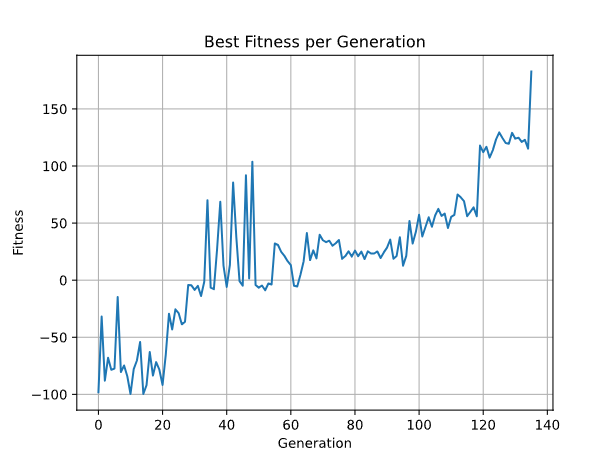
\includegraphics[width=0.7\textwidth]{fitness.png}
	\caption{Best fithess: постепенное увеличение агента указывает на улучшение поведения агента и успешную эволюцию популяции.}
	\label{fig:best_fitness}
\end{figure}

Пример кода для создания графиков динамики метрик:

\begin{lstlisting}[language=Python]
import matplotlib.pyplot as plt

def plot_metrics(fitness_history, loss_history):
    plt.figure(figsize=(10,5))

    # График для среднего фитнеса
    plt.subplot(1, 2, 1)
    plt.plot(fitness_history, label='Best Fitness')
    plt.xlabel('Generation')
    plt.ylabel('Fitness')
    plt.title('Best Fitness per Generation')
    plt.show()
\end{lstlisting}

Этот код строит:
\begin{itemize}
    \item График изменения фитнеса на протяжении поколений, который помогает отслеживать, как улучшается производительность сети.

\end{itemize}

Этот график полезен для визуализации того, как процесс обучения развивается на протяжении нескольких поколений, а также для понимания, насколько эффективно происходит оптимизация сети.

\subsection{Генерация gif-визуализаций}

Для лучшего представления процесса обучения можно создавать gif-анимированные изображения, которые показывают, как агент взаимодействует со средой и как его поведение улучшается с каждым поколением. Эти анимации полезны для наглядного демонстрирования улучшений в стратегии агента.

Пример кода для генерации gif:

\begin{lstlisting}[language=Python]
import imageio

def create_gif(frames, gif_name):
    with imageio.get_writer(gif_name, mode='I') as writer:
        for frame in frames:
            writer.append_data(frame)
\end{lstlisting}

Этот код позволяет создать gif-анимированное изображение из последовательности кадров, например, показывающих агента в различных состояниях во время его обучения в среде. Это является мощным инструментом для визуализации процесса обучения и эволюции агента.

\subsection{Сохранение и загрузка состояния}

Для воспроизводимости экспериментов и анализа прогресса можно сохранять состояние нейронной сети в файл. Это позволяет продолжить обучение с того места, где оно было остановлено, или использовать ранее обученную сеть для тестирования.

Пример кода для сохранения и загрузки состояния:

\begin{lstlisting}[language=Python]
import pickle

def save_network(network, filename):
    with open(filename, 'wb') as file:
        pickle.dump(network, file)

def load_network(filename):
    with open(filename, 'rb') as file:
        return pickle.load(file)
\end{lstlisting}

Этот код позволяет сохранить состояние сети и загрузить его в любой момент, обеспечивая возможность продолжить обучение без потери данных, а также проанализировать прогресс, достигнутый на различных этапах.

Визуализация является важной частью алгоритма NEAT, позволяя отслеживать изменения в структуре сети и динамику метрик, таких как фитнес и потери, на протяжении процесса эволюции. Графики и анимации помогают глубже понять, как работает алгоритм и как он оптимизирует поведение агента в среде. Генерация gif-анимирований и сохранение состояния сети делают анализ и воспроизведение экспериментов более удобным.

\subsection{Видеодемонстрация работы агента}

Gif-анимации с поэтапной эволюцией структуры сети и демонстрацией поведения агента в среде на разных этапах обучения (каждые 50 эпох, а также итоговые результаты) будут приложены к отчёту в виде отдельных файлов. Они позволяют наглядно увидеть не только развитие архитектуры сети, но и качественное изменение траектории посадки аппарата на протяжении обучения.

Ниже приведены скриншоты с демонстрацией походки агента в три ключевых этапа обучения: на 10-й, 50-й и 150-й эпохах. Каждое изображение отражает прогресс в поведении агента при выполнении задачи посадки.

\begin{figure}[H]
	\centering
	\includegraphics[width=0.7\textwidth]{agent.png}
	\caption{Походка на 10-й эпохе. Агент практически не встает на ноги. Он с трудом начинает движение лишь к концу, но уже видны признаки неэффективного контроля, что приводит к сильно отклонённой траектории.}
	\label{fig:landing_epoch10}
\end{figure}

\begin{figure}[H]
	\centering
	\includegraphics[width=0.7\textwidth]{agent_250.png}
	\caption{Походка на 50-й эпохе. Обе ноги заметно начинают движение. Агент корректно поднимает ногу, чтобы двигаться, но всё ещё имеет проблемы с ходьбой.}
	\label{fig:landing_epoch50}
\end{figure}

\begin{figure}[H]
	\centering
	\includegraphics[width=0.7\textwidth]{agent_500.png}
	\caption{Походка на 150-й эпохе. Агент успешно осваивает походку. Он аккуратно и уверено шагает, переворотов нет.}
	\label{fig:landing_epoch150}
\end{figure}

Эти скриншоты иллюстрируют прогресс, который агент демонстрирует в ходе обучения: от неэффективного движения ног и нестабильной траектории в начале, до аккуратной и уверенной походки. Эти изменения отражают улучшение структуры сети и рост её способности к контролю.
\newpage
\section{Развертывание, тестирование и анализ результатов}

Процесс тестирования был реализован с использованием командной строки в среде VS Code. Для запуска программы использовалась команда, которая позволяла как обучать модель, так и проводить её тестирование на обученных весах.

\subsection{Структура проекта}

Проект организован в виде набора Python-модулей и вспомогательных файлов. Основные компоненты:

\begin{figure}[H]
	\centering
	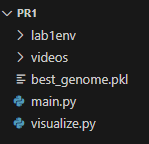
\includegraphics[width=0.7\textwidth]{structure.png}
	\caption{Структура проекта в среде разработки VS Code}
	\label{fig:struct_screenshot}
\end{figure}
\subsection{Основной код: \texttt{main.py}}

\texttt{main.py} представляет собой основной модуль, который содержит реализацию алгоритма NEAT. Включает в себя классы для создания нейронных сетей, мутаций, скрещивания, специализации популяции и коэволюции.

\begin{itemize}
    \item \textbf{NEATConfig:} класс конфигурации, который задает все параметры для эволюции, включая размер популяции, порог для разделения на виды, параметры мутаций и рекомбинации.
    \item \textbf{Gene:} класс для представления связи между нейронами, включая номер инновации, веса связи и статус (включена или выключена связь).
    \item \textbf{NeuralNetwork:} класс для нейронной сети, который управляет созданием сети, её мутацией, а также расчётом выходных данных на основе входных данных.
    \item \textbf{Speciation:} класс для разделения популяции на виды. Он помогает избежать преждевременного вытеснения агентов с новыми структурами.
    \item \textbf{Agent:} класс для представления агента, который взаимодействует с окружающей средой и оценивается по полученному вознаграждению.
    \item \textbf{NEAT:} основной класс, который управляет процессами эволюции популяции, включая мутацию, скрещивание и специализацию.
\end{itemize}

Пример кода для создания популяции агентов:

\begin{lstlisting}[language=Python]
class NEAT:
    def __init__(self, env, config):
        self.env = env
        self.config = config
        self.population_size = config.population_size
        self.agents = [Agent(self.env.observation_space.shape[0], self.env.action_space.shape[0]) for _ in range(self.population_size)]
\end{lstlisting}

\subsection{Визуализация: \texttt{visualize.py}}

Файл \texttt{visualize.py} содержит функции для визуализации ключевых метрик, таких как фитнес, и отслеживания прогресса алгоритма NEAT. Используется библиотека \texttt{matplotlib} для построения графиков.

\begin{itemize}
    \item \textbf{plot\_metrics:} функция для построения графиков динамики изменения фитнеса за поколение. Это помогает наглядно оценить, как увеличивается производительность агентов по мере их эволюции.
\end{itemize}

Пример кода для визуализации фитнеса:

\begin{lstlisting}[language=Python]
import matplotlib.pyplot as plt

def plot_metrics(fitness_history):
    plt.figure(figsize=(10,5))

    # График для среднего фитнеса
    plt.subplot(1, 2, 1)
    plt.plot(fitness_history, label='Best Fitness')
    plt.xlabel('Generation')
    plt.ylabel('Fitness')
    plt.title('Best Fitness per Generation')
    plt.show()
\end{lstlisting}

\subsection{Описание работы алгоритма}

1. Инициализация популяции: Создается начальная популяция агентов, каждый из которых имеет минимальную структуру нейронной сети. Популяция оценивается в среде \texttt{BipedalWalker-v3}, и каждый агент получает своё вознаграждение.

2. Специализация популяции: На основе схожести геномов агентов популяция разделяется на виды с помощью метода \texttt{Speciation}, что помогает сохранить разнообразие в популяции и избежать преждевременной конкуренции между агентов с различными топологиями.

3. Скрещивание и мутация: Процесс скрещивания комбинирует лучшие черты агентов с помощью одноточечного кроссовера, в то время как мутация позволяет добавлять новые нейроны и связи, а также изменять веса существующих связей.

4. Оценка приспособленности: Каждый агент оценивается по вознаграждению, полученному в ходе взаимодействия с окружающей средой. Это вознаграждение используется для вычисления фитнеса.

5. Эволюция: По мере выполнения этих шагов, популяция эволюционирует, улучшая свою способность к выполнению задачи.

\subsection{Сохранение и загрузка состояния}

Для воспроизводимости эксперимента реализована возможность сохранения состояния сети и агентов. Это позволяет продолжить обучение с того места, где оно было остановлено, или протестировать ранее обученную модель.

Пример кода для сохранения состояния:

\begin{lstlisting}[language=Python]
import pickle

def save_network(network, filename):
    with open(filename, 'wb') as file:
        pickle.dump(network, file)

def load_network(filename):
    with open(filename, 'rb') as file:
        return pickle.load(file)
\end{lstlisting}	
	bestgenome.pkl:
	\begin{itemize}
		\item Предобученная сеть (140 эпох)
		\item Используется для демонстрации конечных результатов
	\end{itemize}
	
	Директории:
	\begin{itemize}
		\item \texttt{videos/} --- архив видеозаписей (создается при обучении):
		\begin{itemize}
			\item MP4-анимация работы агента

		\end{itemize}
		\begin{itemize}
			\item Визуализации лучшей сети
			\item PNG-изображения с именем \texttt{agent\_N.png}
		\end{itemize}
		\item \texttt{lab1env/} --- виртуальное окружение Python (исключено из Git)
	\end{itemize}

Проект был размещён на GitHub.   
Ссылка на репозиторий: \url{https://github.com/OKPOIIIKA/NEAT_PR}.

\begin{figure}[H]
	\centering
	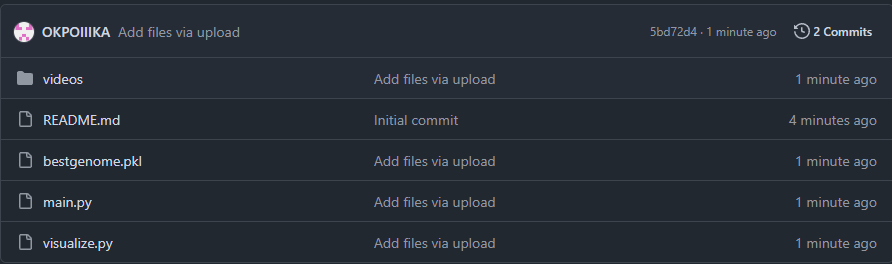
\includegraphics[width=0.7\textwidth]{progect_structure.png}
	\caption{Структура проекта в GitHub}
	\label{fig:project_structure}
\end{figure}

\subsection{Обучение модели}

Для обучения модели использовалась команда CLI в PyCharm с указанными параметрами для количества эпох и размеров скрытого слоя и подпопуляций. Пример команды для запуска обучения на 150 эпох:
\begin{lstlisting}[language=bash]
	for generation in range(150):  
        neat.evolve()
\end{lstlisting}
Программа выводит информацию о прогрессе, включающую лучшее вознаграждение (\textit{best fitness}). Например, на первых эпохах обучение выглядит следующим образом:

\begin{figure}[H]
	\centering
	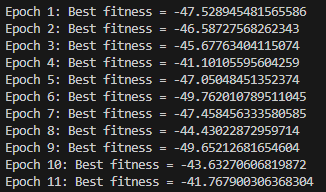
\includegraphics[width=0.7\textwidth]{epoch.png}
	\caption{Скриншот командной строки с результатами обучения на первых эпохах. Программа выводит лучшее вознаграждение каждой эпохи.}
	\label{fig:training_screenshot}
\end{figure}
\subsubsection{Видеодемонстрация работы модели}

Для  проверки качества работы агента была записана видеодемонстрация тестирования, где представлен лучший тестовый эпизод.

Видео позволяет визуально убедиться, что агент после обучения не просто достиг высоких значений reward, но и воспроизводимо демонстрирует требуемое поведение на новых тестовых запусках, что подтверждает реальное качество полученной стратегии управления.

Видео лежит в  папке videos.

На видео видно, что агент:
\begin{itemize}
	\item адекватно корректирует курс;
	\item своевременно шагает;
	\item минимизирует количество лишних манёвров;
\end{itemize}

Это подтверждает, что итоговая модель способна не только обучиться целевой задаче, но и устойчиво применять полученные знания в тестовой среде.
\newpage
\section{Заключение}


В рамках данной работы был реализован и исследован алгоритм нейроэволюции NEAT для обучения нейронной сети на задаче управления агентом в среде \texttt{BipedalWalker-v3}. Был выполнен полный цикл разработки: от создания модульной структуры кода и реализации алгоритма NEAT до визуализации структуры сети и анализа результатов обучения.

Проведённые эксперименты показали, что метод NEAT обеспечивает эффективное и устойчивое обучение агентам с различными архитектурами нейронных сетей, начиная с простых структур и постепенно усложняя их по мере необходимости. Эволюция сети с добавлением нейронов и связей позволяет адаптировать архитектуру для выполнения задачи в условиях динамичной среды. Прогресс в процессе эволюции наглядно прослеживается как по динамике целевых метрик (среднее вознаграждение и loss), так и по визуализации структуры сети, что подтверждает способность алгоритма NEAT улучшать качество решения задачи.

Результаты тестирования подтверждают высокую эффективность подхода: агент, обученный в течение 150 поколений, стабильно выполняет задачу управления движением в среде \texttt{BipedalWalker-v3}, демонстрируя улучшение в вознаграждении и эффективности стратегии. Средние значения вознаграждения в тестовых эпизодах подтверждают, что сеть способна обобщать навыки и уверенно действовать в различных сценариях среды.

Кроме того, была реализована система сохранения и загрузки состояния нейронной сети, что обеспечивает воспроизводимость результатов и удобство для дальнейших экспериментов. Визуализация, включающая отображение структуры сети и графики динамики метрик, значительно помогает в анализе работы алгоритма и поведении агента.

Таким образом, алгоритм NEAT продемонстрировал свою эффективность при решении задач с непрерывным управлением и может быть использован для других сложных задач в области обучения с подкреплением, где традиционные методы обучения могут быть недостаточно эффективными. Нейроэволюция, и в частности NEAT, остаётся перспективным инструментом для построения адаптивных интеллектуальных систем, способных решать задачи с высокой размерностью и сложной динамикой.
\newpage
% Список литературы
\section*{Список использованной литературы}
\begin{enumerate}
    \item Лекция 9. Алгоритм NEAT. Томский политехнический университет, 2025.
\end{enumerate}

\end{document}
